\chapter{Data Collection}

\section{The MultiplEYE Project}

\subsection{Overview}
The MultiplEYE project is a research initiative that aims to bring together researchers from various fields working with eye-tracking data in multiple languages. The name MultiplEYE is a play on the words "multiple" and "eye", reflecting the project's focus on eye-tracking data in multiple languages. One of the main goals of the project is to create a large multilingual eye-tracking dataset that can be used to study human reading from a psycholinguistic perspective and to improve various natural language processing tasks.

\subsection{Experiment Design}
The MultiplEYE experiment is designed to collect eye-tracking data from participants reading a set of texts in their native language. The experiment consists of two main parts: a reading task and a comprehension task. The participant sits in a chair at a desk with their chin and forehead resting on a support platform to prevent them from moving their head. On the desk there is a monitor displaying the text the participant has to read. Below the monitor, the eye-tracking device is tracking their eye movements. 

\section{Stimuli}
In total, there are 13 texts in the main experiment, 2 practice texts, and 2 back-up texts. After reading each text stimulus, participants are asked to answer some comprehension questions. At the end of the experiment, participants have to complete a questionnaire regarding basic information about themselves and their reading habits.

The texts are selected from a variety of genres: popular science (PopSci), literary (Lit), argumentative (Arg), institutional (Ins), and encyclopedic (Enc). The main 13 texts are: 1 - PopSci\_MultiplEYE, 2 - Ins\_HumanRights, 3 - Ins\_LearningMobility, 4 - Lit\_Alchemist, 6 - Lit\_MagicMountain, 8 - Lit\_Solaris, 9 - Lit\_BrokenApril, 10 - Arg\_PISACowsMilk, 12 - Arg\_PISARapaNui, and 13 - PopSci\_Caveman. The 2 practice texts are: 7 - Lit\_NorthWind, and 11 - Enc\_WikiMoon. The 2 back-up texts are: 14 - Lit\_HarryPotter, and 5 - Lit\_EmperorClothes.

The texts used in the MultiplEYE experiment are originally in English, and so if someone wants to run the experiment and collect eye-tracking data in another language, they have to translate the texts. The project provides a set of guidelines for the translation process. 

For the Romanian translation, some of the texts were replaced with an already existing Romanian translation, for example the texts that were taken from books, while others were translated by Sergiu Nisioi using machine translation. I then edited the translations to make them more fluent and natural. The comprehension questions were also initially translated using machine translation, but needed significant editing.

After translating the stimuli, in order to run the experiment, images with the texts and questions have to be generated. I used the \textit{MultiplEYE Image Generation Software} \cite{Jakobi2025_MultiplEYE} to generate the images and other necessary files for the experiment.

\section{Running the Experiment}
In order to run the experiment, the MultiplEYE project provides a software package \textit{MultiplEYE Experiment Implementation} \cite{MultiplEYE_ExperimentImplementation2025}. 

An eye-tracking device is required to run the experiment. The University of Bucharest has an EyeLink 1000 Plus eye-tracker at the Faculty of Psychology and Educational Sciences, which I used to run the experiment. In order to properly utilize the eye-tracker, I familiarized myself with the device using the documentation provided by the manufacturer \cite{EyeLink1000PlusUserManual}. The eye-tracker is connected to a computer that runs the MultiplEYE Experiment Implementation software. The participant sits in front of the eye-tracker and reads the texts displayed on the monitor. The eye-tracker records their eye movements while they read.

The experiment was run with 4 participants, all of them native Romanian speakers. The experiment took about 1-2 hours for each participant to complete. All participants were volunteers and were informed about the purpose of the experiment and how their data would be used. 

\section{Pymovements}
The MultiplEYE project uses the \textit{Pymovements} library \cite{Krakowczyk2023_pymovements} for extracting eye-tracking data from the raw data collected by the eye-tracking device. First, I convert the raw data file from the EyeLink 1000 Plus eye-tracker from the EDF format to ASCII using the \textit{EDF2ASC} tool provided by the eye-tracker manufacturer. The resulting ASCII file contains the raw eye-tracking data, which is then processed using the \textit{Pymovements} library, which calculates the fixations, saccades, and other eye movement events from the raw data. Then, the fixations are mapped to the text stimuli in order to obtain the reading times for each word in the text.

The eye-tracking experiment records the eye movements both during the reading task and during the comprehension task. Since I want to focus on ppredicting the total reading time for words during normal reading, I only keep the data from the reading task.

\section{Mapping Words to Sentences}
Since for some of the features I want to extract I need to know the sentence each word belongs to, I need to map the words to the sentences in the text. For this, I created some auxiliary functions and files and split the texts from each screen into sentences using a regex: 
\begin{verbatim}
    (?<=[.!?:])\s+|(?<=\n)\s*|(?<=\.”)
\end{verbatim}
This regex splits the text into sentences by matching the following patterns:
\begin{itemize}
    \item A period, exclamation mark, question mark, or colon followed by one or more whitespace characters.
    \item A newline character followed by zero or more whitespace characters.
    \item A period followed by a closing quotation mark.
\end{itemize}

\section{TRT Data}
Before extracting features or training models, I looked at the data collected from the experiment. The data consists of the total reading time (TRT) for each word in the text, which is the sum of the reading times for all fixations on that word. The TRT is calculated by summing the durations of all fixations on a word, which gives an indication of how long the participant spent reading that word.

The TRT data for each participant is stored in a CSV file with columns for the participant ID, the text ID, the word ID, the word itself, the sentence ID, the sentence itself, the word index in the sentence, and the TRT for that word. The TRT is measured in milliseconds. I averaged the TRT across all participants for each word in the text, which gives a more reliable estimate of the reading time for each word. 

However, there are some differences between the stimuli of each of the participants. The first two participants had slightly differently translated texts, while the last two participants read the final version of the texts. I used the final version of the texts and simply excluded metrics from the first two participants for sentences that were not identical to the final version. Another important difference is that during the experiment with the first participant, the eye-tracking computer malfunctioned and shut down, which resulted in a stimuli, 10 - Arg\_PISACowsMilk, not being read at all. Luckily, the data for the other texts was still collected, so I could use that data for the analysis.

The figure \ref{fig:trt_data} shows a histogram of the TRT data, which gives an overview of the distribution of reading times across the dataset. As is visible in the histogram, a lot of words have a total reading time of 0 milliseconds, which means that the participant did not fixate on those words at all. This is expected, as some words in the text may be skipped or read very quickly without any fixations. The histogram also shows that there are some words with very high TRT values, which indicates that those words were read more carefully or were more difficult to process.

\begin{figure}
    \centering
    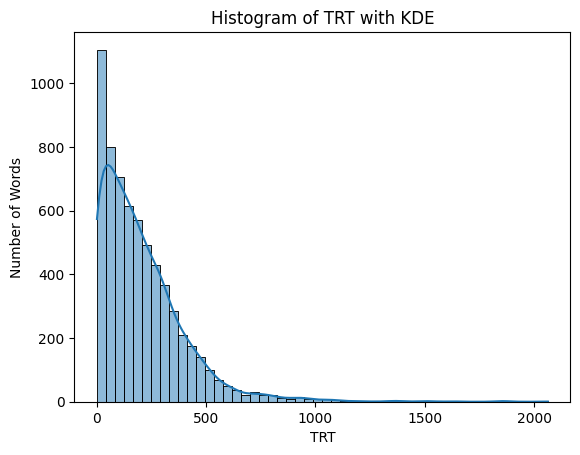
\includegraphics[width=0.8\textwidth]{images/TRT_histogram_KDE.png}
    \caption{Histogram of Total Reading Time}
    \label{fig:trt_data}
\end{figure}